\chapter{Software implementation}
%Add introduction to chapter
The software implementation chapter describes ROS (Robot Operating System) along with the implemented packages and algorithms. The first package that is looked at is the TF package that is used to transform the readings between the different sensors. The two major packages installed are leg\_detector and face\_detector, which are used to locate the people in proximity of the sensors. \\

The description of the robot and transformation between its coordinate frames are first used by specifying the placement of the different parts and their relationship. Then the depth image and laser scans are used for face detection and leg detection, respectively. They are used to keep track of the customer who uses a the robot in the hypermarket. The output of both detections are fused to give one Cartesian position of the person that is used for velocity control depending on the distance between the robot and the customer who is using it. The robot moves in the hypermarket by using the "move\_base" package. It uses the laser scan to localise itself in a known map and moves to a desired location in it while avoiding obstacles. If the customer is still following the robot, the robot keeps moving towards the desired location. This can be seen in figure \ref{fig:dia}.

\begin{figure}[H]
    \centering
    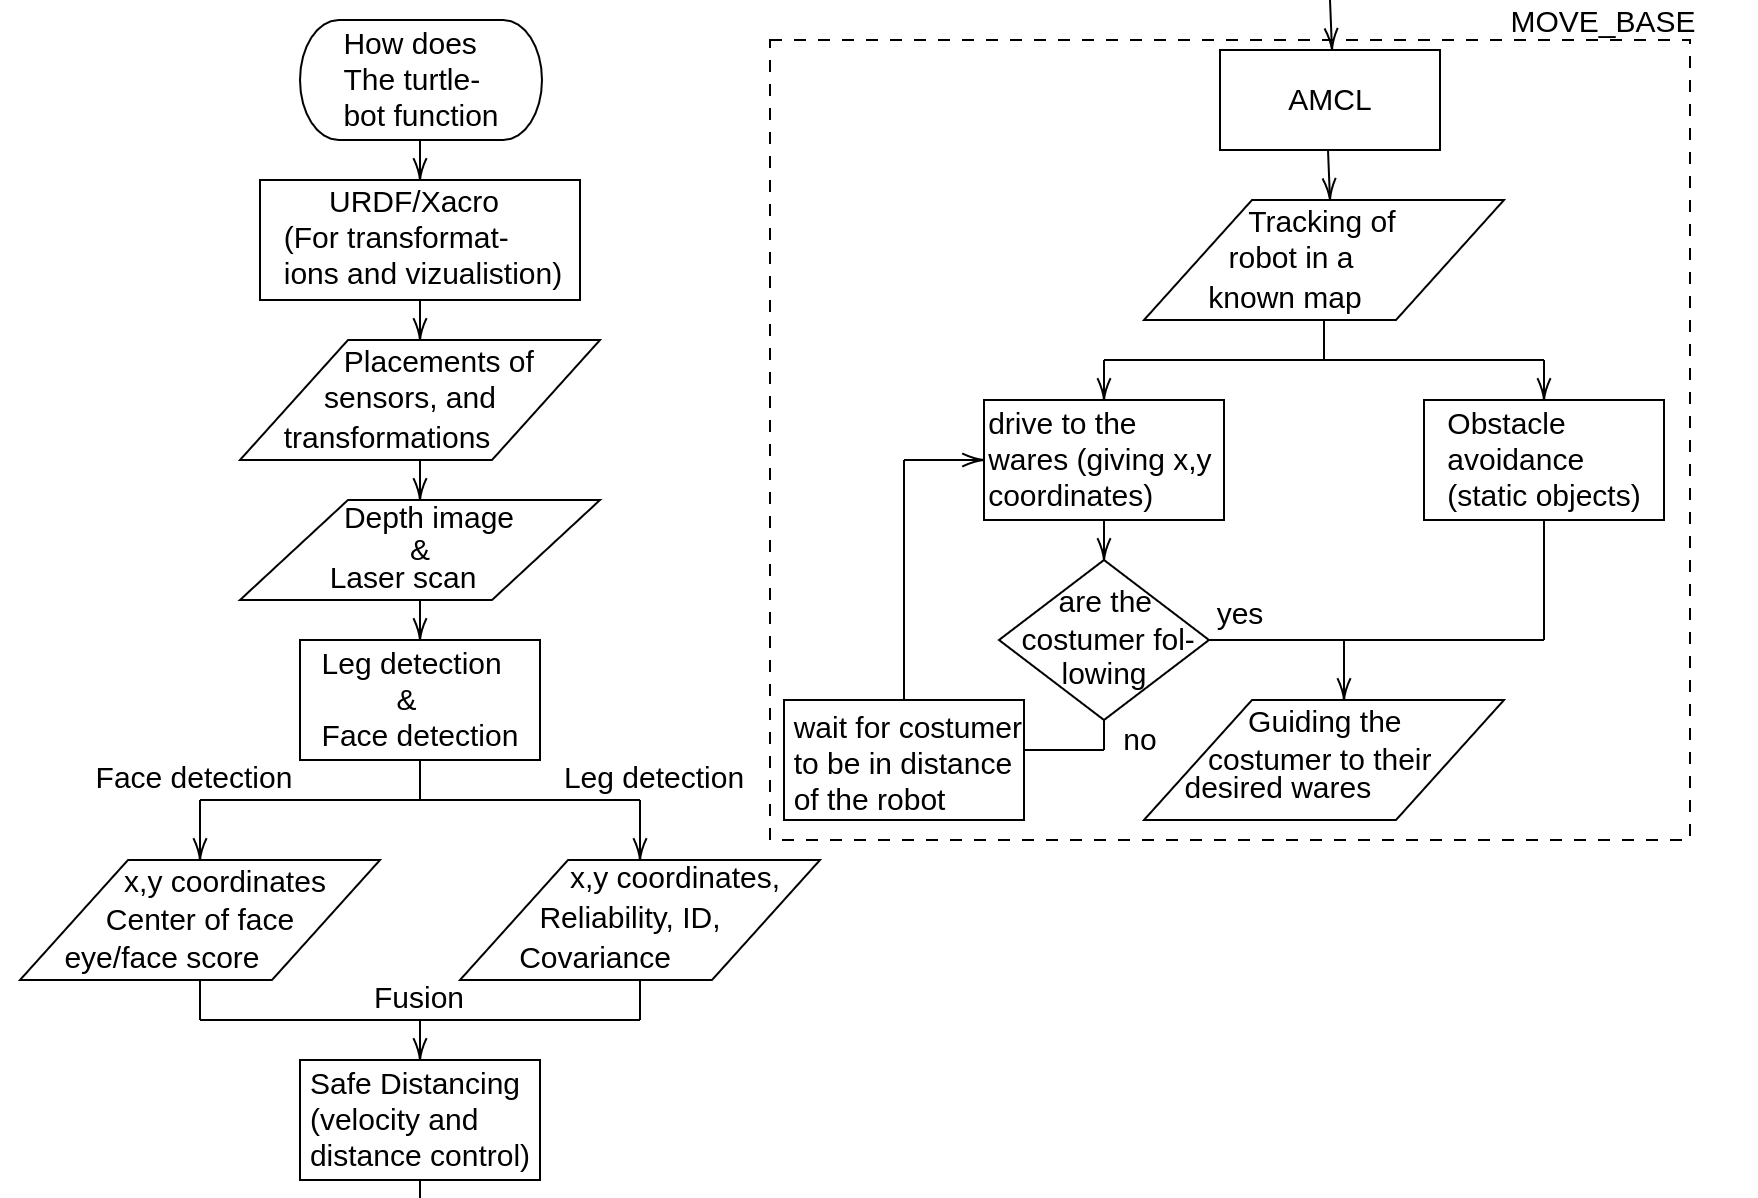
\includegraphics[width=1\textwidth]{figures/imp1.png}
    \caption{This flowchart describes how the implementation of the different data acquisitions, algorithms and sensors is done. The first process to be undergone is the URDF, so that the algorithm will know where the different sensors are located in relation to each other, then from the image and laser captures the two main algorithms will be run "face detection" and "leg detection". These two are running parallel and when outputs is received it will be fused so that a person might be perceived from this. When the person in the FOV is tracked a velocity control can begin, where the safe distance is described as in the social space, see fig \ref{fig:hall}, and MOVE\_BASE can commence. MOVE\_BASE uses the AMCL, which can be read about in the section about MOVE\_BASE. This MOVE\_BASE tracks itself in a map and should drive to the wares while avoiding obstacles. The last  implemented part is velocity control that ensures, the robot lowers its velocity or stops when the costumer following is not in the measured distance. This can be read in the section revolving the velocity-distance. If all of the above is successful then the guiding is undergoing or done.}
    \label{fig:dia}
\end{figure}

\section{ROS}\label{sec:ROS}
Robot Operating System (ROS) is an open-source software framework used for developing robotics software. It provides hardware drivers for a variety of sensors, and has a vast number of libraries, tools, and different algorithms that ease the task of programming robots, whether it is mobile robots or manipulators. It also provides visualisation and simulation tools. The core function of ROS is passing messages, which is done using publisher and subscriber communication paradigm.
Since ROS uses publisher and subscriber methods to exchange messages, a third component known as ROS master is used to filter and distribute the published messages to the corresponding subscriber.
Using ROS, processes communicate with each other through a peer-to-peer connection which is established by the ROS master. This network is known as ROS computational graph, where processes can be distributed across multiple machines or running on the same. ROS master keeps track of the running processes, also known as nodes, and handles name registration of them. ROS routes the messages published by the nodes to one another on a specific topic, where topics are named buses used for transferring data between nodes.\\
There are many reasons for using ROS, which include support for different programming languages such as C++, Python, Java, Lua and many others. Library integration is yet another advantage as many popular third-party libraries are supported such as OpenCV and Point Cloud Library (PCL). Scalability in the form of cloud computing is also possible using ROS in order to perform compute-intensive tasks. ROS also has tools for logging and playback of data in addition to tools for testing to find bugs in the code and to ensure its quality.\cite{ROScorecomponent}\\
A package this project has surrounded its algorithms around, is the "ros-people", and this package includes two different algorithms, such as "face-detection" and "leg-detection". However, before these algorithms can be dove into, a description of how the different sensors is placed is necessary.